\documentclass[10pt,twocolumn,letterpaper]{article}

%% Latex documents that need direct input
%
% ACPR template packages
\usepackage{acpr}
\usepackage{times}
\usepackage{acro}
\usepackage{epsfig}
\usepackage{amsmath}
\usepackage{amssymb}
\acresetall
%  The following command loads a graphics package to include images
%  in the document. It may be necessary to specify a DVI driver option,
%  e.g., [dvips], but that may be inappropriate for some LaTeX
%  installations.
\usepackage[]{graphicx}

% In order to include files without having a clear page using \include*,
% the newclude package is required
\usepackage{newclude}

% Required for acronyms
%use \acresetall to reset the acroyms counter
%macros=True, allows for calling \myTriger rather than \ac{myTriger}
%\usepackage[single=true, macros=true, xspace=true]{acro}

% Use biblatex to manage the referencing
%
\usepackage[style=ieee, backend=biber, backref=true]{biblatex}

% Include other packages here, before hyperref.

% If you comment hyperref and then uncomment it, you should delete
% egpaper.aux before re-running latex.  (Or just hit 'q' on the first latex
% run, let it finish, and you should be clear).
\usepackage[%pagebackref=true,
            breaklinks=true,
            letterpaper=true,
            colorlinks,
            bookmarks=false,
           ]{hyperref}

% Clever cross referencing. Using cleverref, instead of writting
% figure~\ref{...} or equation~\ref{...}, only \cref{...} is required.
% The package interprates the references and introduces the figure, fig.,
% equation, eq., etc keywords. \Cref forces first letter capital.
% >> WARNING: This package needs to be loaded after hyperref, math packages,
%             etc. if used.
%             Cleveref is recomended to load late
\usepackage{cleveref}

% To create random text use lipsum
\usepackage{lipsum}
%\usepackage{translations}        % contains the latex packages
\title{Tackling the Curse of Data Imbalancing for Melanoma Classification}

\author{Mojdeh Rastgoo, Guillaume Lema\^itre, Rafael Garcia\\
Universitat de Girona\\
Campus Montilivi, Edifici P4, 17071 Girona\\
% For a paper whose authors are all at the same institution,
% omit the following lines up until the closing ``}''.
% Additional authors and addresses can be added with ``\and'',
% just like the second author.
% To save space, use either the email address or home page, not both
\and
Joan Massich, Olivier Morel, Fabrice M\'eriaudeau, Franck Marzani\\
Universit\'e de Bourgogne Franche-Comt\'e\\
12 rue de la Fonderie, 71200 Le Creusot\\
}
             % contains the Title and Autor info
%%%%%%%%%%%%%%%%%%%%%%%%%%%%%%%%%%%%%%%%%%%%%%%%%%%%%%%%%%%%% 
%>>>> uncomment following for page numbers
% \pagestyle{plain}    
%>>>> uncomment following to start page numbering at 301 
%\setcounter{page}{301} 
      % contains package and variables init.
%% Acronym definition example using glossaries package
%% \usepackage{acro} is required
%% 
%% For a powerful usage of the acro package look at http://tex.stackexchange.com/questions/135975/how-to-define-an-acronym-by-using-other-acronym-and-print-the-abbreviations-toge

\DeclareAcronym{cnn}{
  short = CNN,
  long = Condensed Nearest Neighbour
}

\DeclareAcronym{nn}{
  short = NN,
  long = Nearest Neighbour
}

\DeclareAcronym{oss}{
  short = OSS,
  long = One-Sided Selection
}

\DeclareAcronym{smote}{
  short = SMOTE,
  long = Synthetic Minority Over-sampling TEchnique
}

\DeclareAcronym{enn}{
  short = ENN,
  long = Edited Nearest Neighbour
}

\DeclareAcronym{svm}{
  short = SVM,
  long = Support Vector Machines
}

\DeclareAcronym{cad}{
  short = CAD, 
  long = Computer-Aided Diagnosis
}

\DeclareAcronym{clbp}{
  short = CLBP,
  long = Completed Local Binary Pattern
}
\DeclareAcronym{lbp}{
  short = LBP,
  long = Local Binary Pattern
}
\DeclareAcronym{rf}{
  short = RF,
  long = Random Forests
}

\DeclareAcronym{ncr}{
  short = NCR,
  long = Neighborhood Cleaning Rule
}

\DeclareAcronym{se}{
  short = SE,
  long = Sensitivity
}

\DeclareAcronym{sp}{
  short = SP,
  long =  Specificity
}

\DeclareAcronym{wracc}{
  short = WRacc,
  long = Weighted Relative Accuracy
}

\DeclareAcronym{fpr}{
  short = FPR,
  long = False Positive Rate
}

\DeclareAcronym{nm}{
  short = NM,
  long = NearMiss
}

\DeclareAcronym{nm1}{
  short = NM1,
  long = NearMiss-1
}

\DeclareAcronym{nm2}{
  short = NM2,
  long = NearMiss-2
}

\DeclareAcronym{nm3}{
  short = NM3,
  long = NearMiss-3
}

\DeclareAcronym{os}{
  short = OS,
  long = Over-Sampling
}

\DeclareAcronym{ros}{
  short = ROS,
  long = Random Over-Sampling
}

\DeclareAcronym{us}{
  short = US,
  long = Under-Sampling
}

\DeclareAcronym{rus}{
  short = RUS,
  long = Random Under-Sampling
}

\DeclareAcronym{cus}{
  short = CUS,
  long = Clustering Under-Sampling
}

\DeclareAcronym{bd}{
  short = BD,
  long = Barrel Deformation
}

\DeclareAcronym{rdgm}{
  short = RDGM,
  long = Random Deformation using Gaussian Motion 
}

\DeclareAcronym{tl}{
  short = TL,
  long = Tomek Link 
}      % contains the acronims 

\acprfinalcopy % *** Uncomment this line for the final submission
\def\acprPaperID{438} % *** Enter the acpr Paper ID here
\def\httilde{\mbox{\tt\raisebox{-.5ex}{\symbol{126}}}}
% Pages are numbered in submission mode, and unnumbered in camera-ready
\pagestyle{empty}


%% Select inputing only one part of the document
%\includeonly{content/intro/intro}   % the file wihtout .tex
%\includeonly{content/other/other_content}
 
\addbibresource{references.bib}

\begin{document} 
\maketitle 

\begin{abstract}
Real-time digital image/video processing is a widely used computer vision/graphics technique. For the purpose of high performance designs, variant computation platforms are make available to the engineers with affordable prices. However, these sophisticated devices usually require a specific implementation framework to transplant the desired algorithm from software environment into hardware environment. Since this process is quite effort-consuming, finding a new approach that can accelerate the development cycles the image/video processing applications becomes a new challenge.
This work focus on fast SW/HW Co-design Framework for real-time image/video processing. After a carefully methodology exploration to the currently available hardware platforms, we select Field Programmable Gate Arrays (FPGAs) as our target platform due to its high performances in terms of efficiency-cost. Next, we base our research on an improved C-synthesis design flow, and development a novel Code and Directive Manipulation Strategy for High-Level Synthesis (CDMS4HLS). Finally, intensive experiment demonstrate that, compared with the other similar approaches, our method can essentially reduce the effort of the development cycles and potentially improve the performances of final implementations.
%\keywords{\acl{dme}, \acl{oct}, \acs{dme}, \acs{oct}, \ac{lbp}.}
\end{abstract}

\section{Introduction}
\label{sect:introduction}
In image science, image/video processing is one of the applications of signal processing technics. It includes methods for analyzing, processing or treating images. The motivation of this field is to improve the target images to meet the requirements in visual, mental or other technical terms. Since images are usually stored in digital format currently, image/video processing refers to digital image/video processing in most cases.

With the fast development of digital signal processing technics, image/video processing is widely used in variant fields, such as satellite image analyzing, computer-aided medical diagnosis, face identification, microscope image processing and car barrier detection, etc.. Meanwhile, the algorithms for image processing become increasingly complex and computationally intensive. For the purpose of performances, series of computation platforms are developed and made available with an affordable price, i.e. Graphics Processing Unit (GPU), Digital Signal Processor (DSP), Centeral Processing Unit (CPU) and FPGA etc.. Since these sophisticated devices have quite different architectures, engineers have to transplant their designs from software environments (i.e. Matlab, OpenCV and C/C++) into specific hardware environments within different development frameworks, i.e. Message Passing Interface (MPI) for CPU, Compute Unified Device Architecture (CUDA) for GPU or Hardware Description Language (HDL) for FPGA etc..

Implementing a design from software environment into hardware environment is a painful and effort-consuming process. This is because the languages used for hardware configuration are usually low-abstract, which are inconvenient for algorithm specification. In order to improve both productivity and performances of the desired designs, many image research and development communities base their works on a streamlined design flow, known as SW/HW Co-design.

SW/HW Co-design is an important approach to ensure an efficient final implementation of the product. In order to further improve the research and development productivity, series of Computer Aided Software Engineering (CASE) based software
tools are put into operation. Moreover, the progresses of software engineering increasingly provide opportunities to seek new design methodology with better productivity.

We focus our work on the SW/HW Co-design methodology exploration for real-time image/video processing development. The main purpose of this research project is to propose a new methodology to quickly conceive and realize high-performance implementations for real time image/video processing with high adaptability capacity. According to the achievements of a careful bibliography study, we base the new approach on the High-Level Synthesis (HLS) SW/HW Co-design framework for FPGAs, and improve it according a source-to-source compiler. During this effort, a novel CDMS4HLS is developed.

In this new SW/HW Co-design framework, we provide multiple advantages:
\begin{itemize}
\item[-] The new approach provides a C/C++ development environment, which allows engineers to realize rapid prototyping of signal and image processing on target devices ignoring completely hardware aspects.
\item[-] The new approach performs an open and adaptive framework which allows parallel optimizations in different levels, i.e. FLP, LLP, ILP and DLP etc.. Nevertheless, the optimizations can easily made and don't require much hardware knowledge.
\item[-] Comparing with the conventional methodologies, the new approach doesn't make any negative effects to the designs in terms of power-efficiency, and the loss of accuracy or cost-efficiency due to the hardware devices are acceptable in most cases if it exists.
\end{itemize}

Experiment results demonstrate that our approach can provide the engineers a quite software-convenient environment for development and optimization as well. Furthermore, our approach can make more efficient use of the hardware resources than the other similar FPGA design flows and provide higher performances than the implementations on the other computation platforms.

After the introduction section, the remains of this thesis is organized as follows: Section \ref{sect:related works} explores the state of the art of HLS based FPGA design flows, Section \ref{sect:Souce-to-Source compilation based HLS design flow} presents the proposed code and directive manipulation strategy for it, Section \ref{sect:experiments} discusses the experiment results and a conclusion is given in the final section.

\section{Related works}
\label{sect:related works}
Over the past twenty years, High-Level Synthesis (HLS) technique has made great progress. Recently, some robust and mature HLS SW/HW Co-design development frameworks have been made available to engineers, i.e. Vivado\_HLS of Xilinx \cite{59} and Catapult C Synthesis Work Flow \cite{60}. These convenient tools allow to specify targeted hardware behaviour in high abstract levels rather than RTL, and then create the Hardware Description Language (HDL) specification of desired FPGA implementations from its software prototype through an automatical C-to-RTL transformation. This approach can greatly accelerate the developments by freeing the designers from the boring work of hardware implementing \cite{30}.

        \begin{figure}[t]
        \centering
        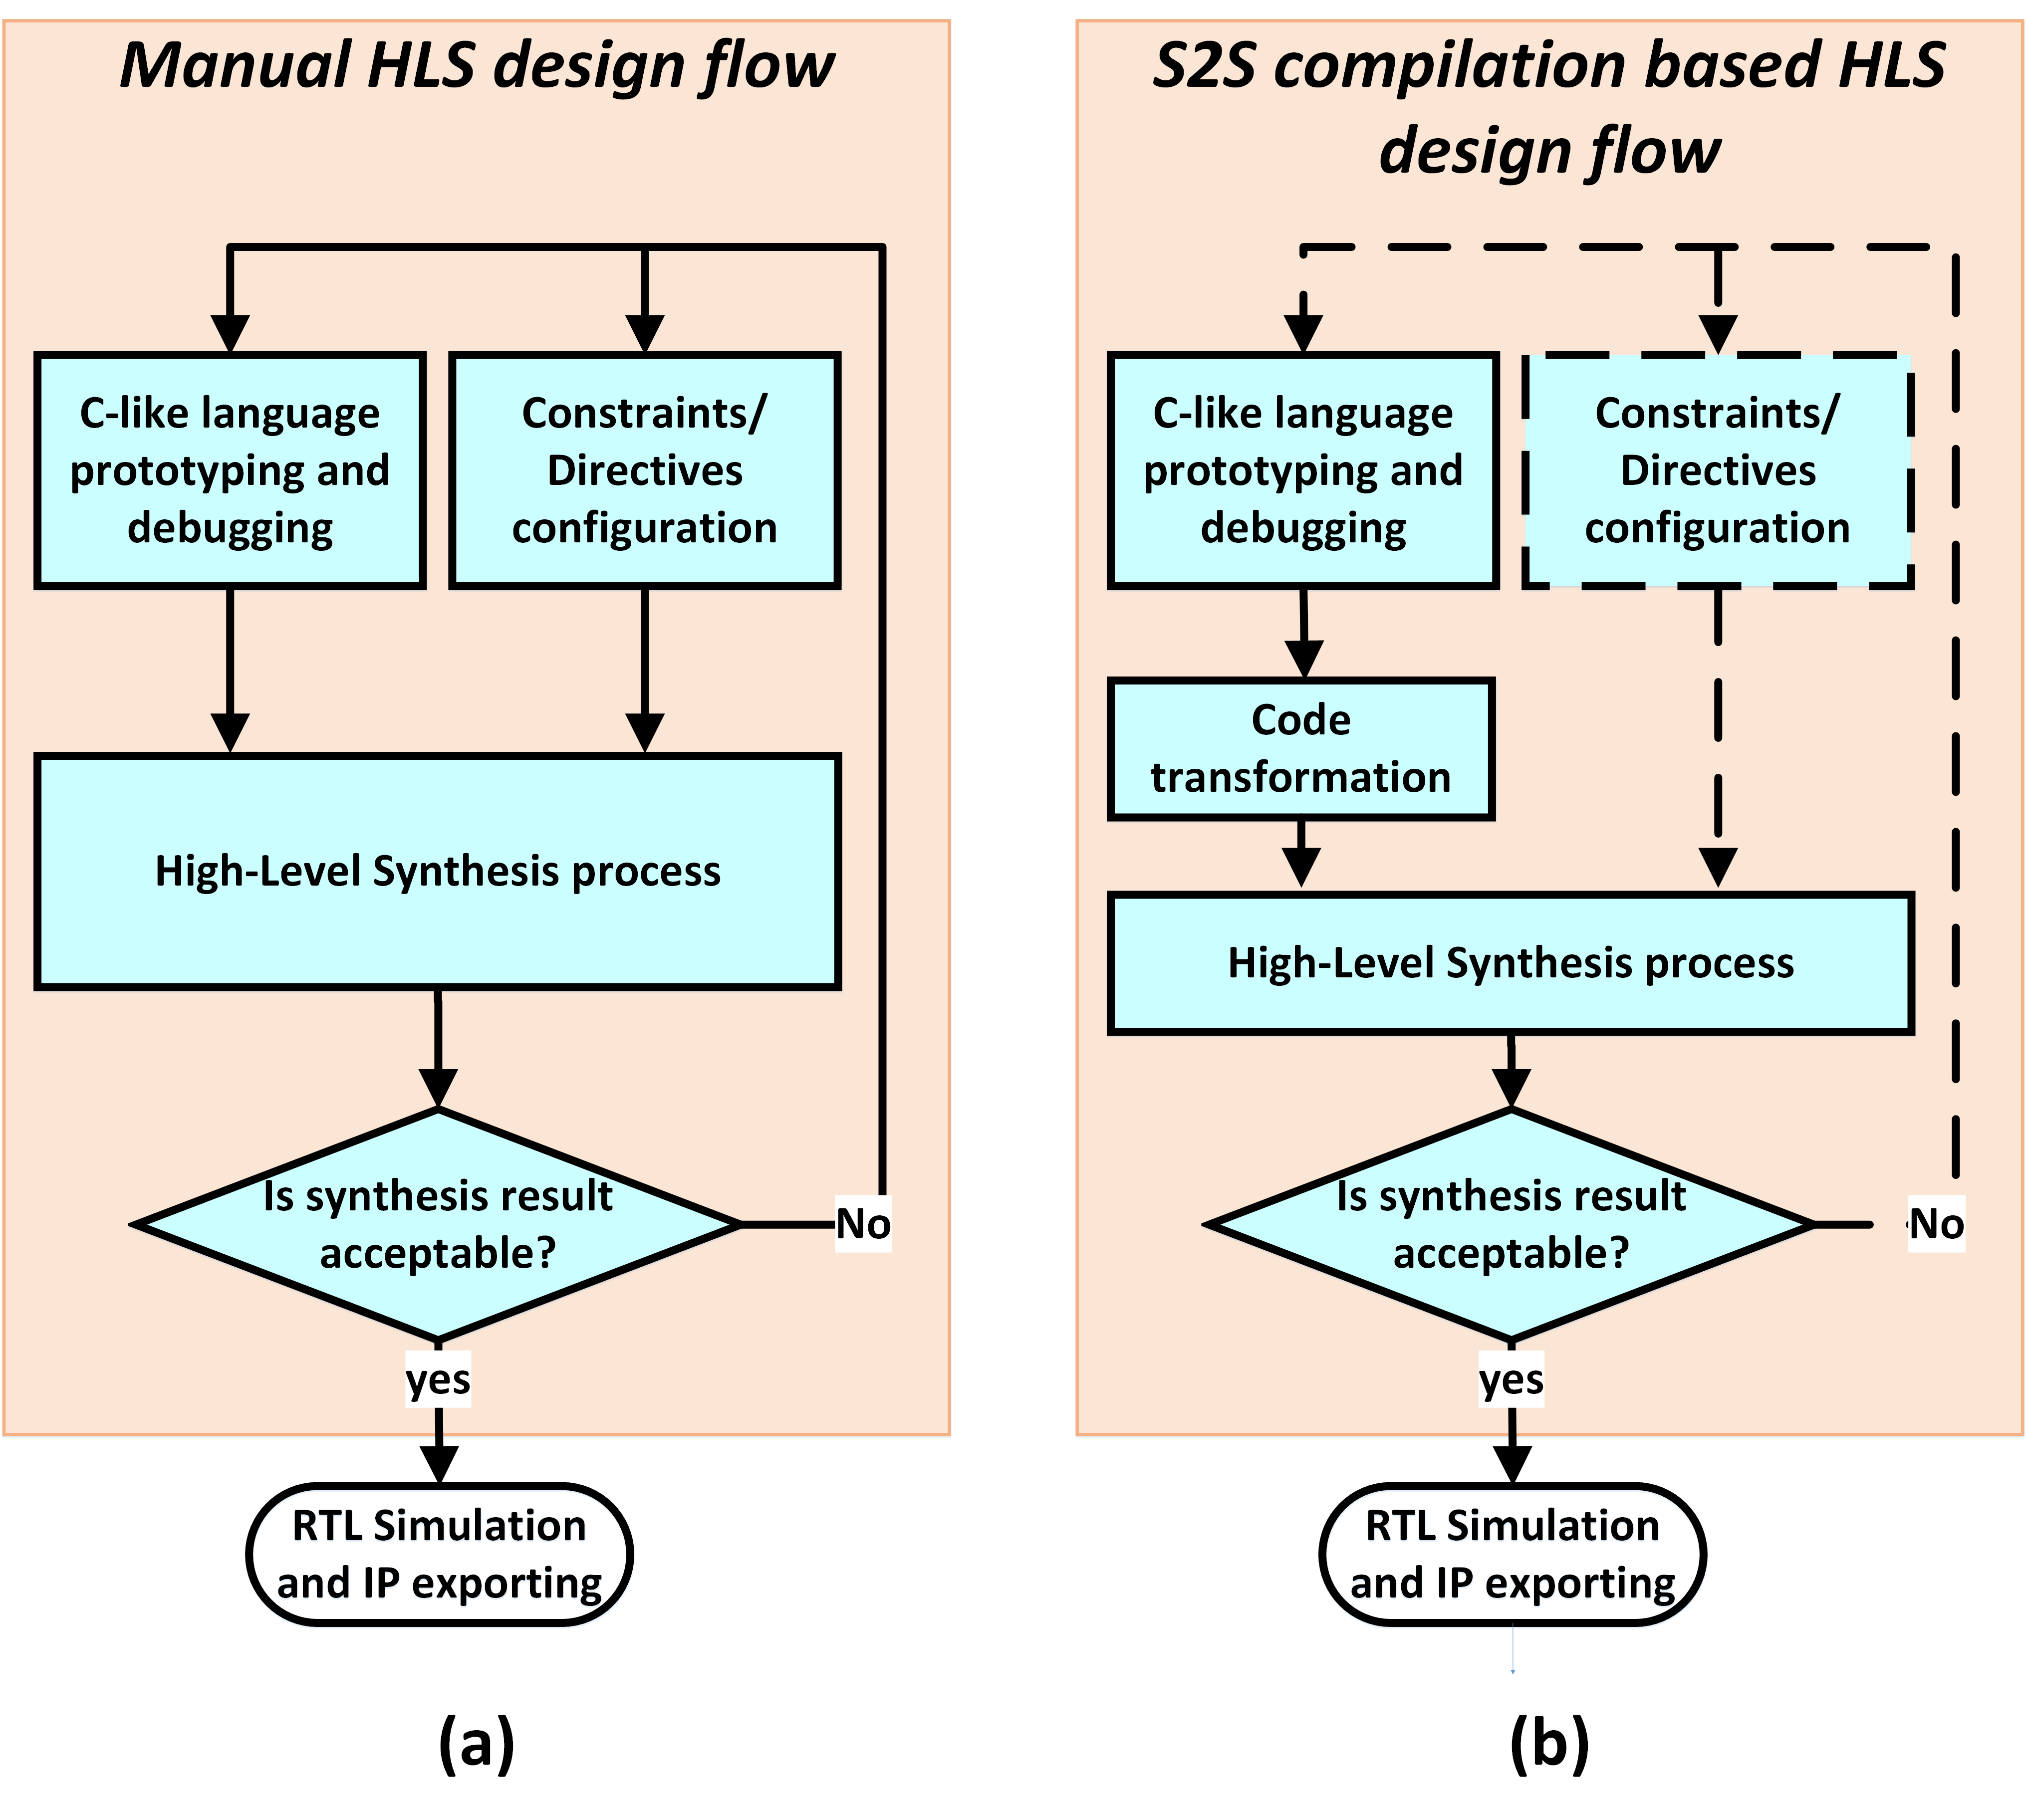
\includegraphics[width=\linewidth]{DesignFlow4HLS.png}
        \caption{Manual and source-to-source compiler based HLS design framework.}
        \label{DesignFlow4HLS}
        \end{figure}

Fig.\ref{DesignFlow4HLS}-(a) illustrates the framework of HLS-based FPGA designs. First of all, designers specify the software prototype of targeted algorithm in C-like languages and debug it in a test bench using common C compilers. Next, the confirmed code is imported into a HLS tools as original sources for C-to-RTL synthesis. During this process, the designers configure the synthesis constraints/directives to make their implementations suitable for different design requirements. At last, the generated HDL specification is simulated by a RTL simulator like ModelSim, and then exported as IP-blocks. This approach doesn't require specific knowledge of both software and hardware, so users can concentrate their attentions only on the algorithm specifications in high abstract levels. However, with the widespread of HLS tools in the ES (Embedded System) world, more issues related to time control, execution speed and consummation etc. emerge. In order to find out the best design solution, designers have to configure repeatedly the directives, and sometimes even have to re-specify their algorithms to ensure the input sources to be detectable by HLS processes. This is a quite painful and effort-costly job even for an experienced SW/HW Co-design engineer.

The issue of HLS design flow discussed above is caused by three major reasons: a) the C-language suitable to HLS tools is just a subset of C-like languages, we therefore cannot benefit to all the C advantages during the algorithm specification, b) different designers and algorithms may result in different code structures and styles, so the data dependency of input sources sometimes can't be perfectly determined by scheduling process for optimization and c) the existing synthesis tools provide dozens of directives for hardware constraints which requires the designers to be quite familiar with synthesis tools. For the purpose to further simplify the development cycles, a source-to-source (S2S) transformation based HLS design flow was developed (see Fig.\ref{DesignFlow4HLS}-(b)). In this new framework, a S2S compiler is inserted between the software prototyping and synthesis process. In contrast with the manual specification and configuration, this bridge tool automatically transforms the original code into the sources more efficient. For example, Alle et al. propose an efficiency improvement approach for loop pipelining in HLS through a semi-automatic source-to-source transformation in \cite{57}.

\section{souce-to-source compilation based HLS design flow}
\label{sect:Souce-to-Source compilation based HLS design flow}
C-to-RTL synthesis is the key technique of HLS. It offers many opportunities to optimize the designs in different hierarchies, including function level, loop level, instruction level and data level etc.. Therefore how to perform an efficient source code and perfectly combine these optimization strategies together becomes a new challenge for engineers. This is usually a painful and time-costly work because it has to be repeated several times until an acceptable, even if the best solution is found. Thus, some C-to-C compilers emerges. That effectively raise the productivity of such design by automatically improving the efficiency of manual code.

This section describes a C-to-C compilation strategy for HLS, CDMS4HLS, which can streamline the code optimization process. Unlike some existing research productions, we base this work on the special characteristics of HLS in terms of synthesis process rather than borrow some achievements from other efforts about parallel computing for high performance computers. The over-all structure of CDMS4HLS is shown in Fig.\ref{CDMS4HLS}, which consists of function inline, loop fusion, symbolic expression manipulation, loop unwinding and array reshape. These 5 steps are effected on input source code in a proper order for the purpose to enable each optimization method to make a maximum effectiveness.

        \begin{figure}[t]
        \centering
        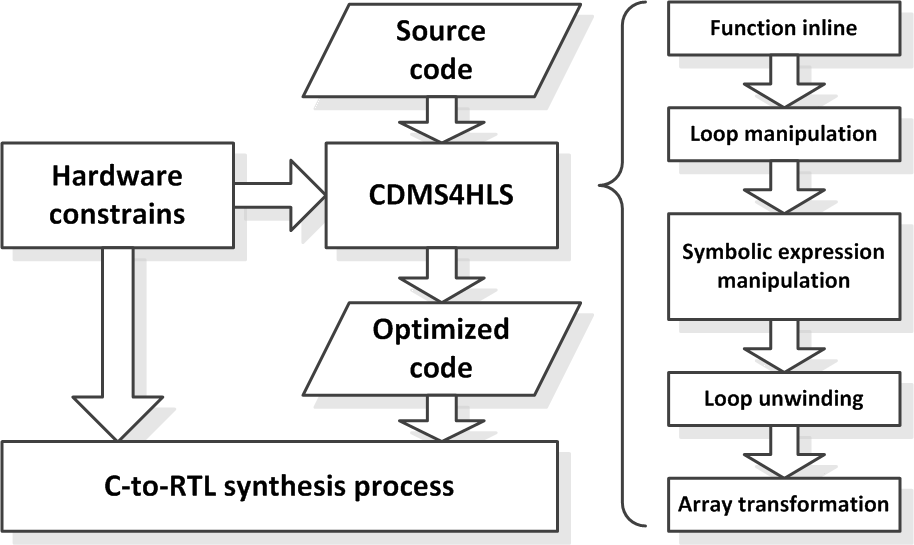
\includegraphics[width=0.8\linewidth]{CDMS4HLS.png}
        \caption{CDMS4HLS compilation process.}
        \label{CDMS4HLS}
        \end{figure}

\section{Experiments}
\label{sect:experiments}
\label{Comparison experiment}
    \begin{figure}
    \centering
    % Requires \usepackage{graphicx}
    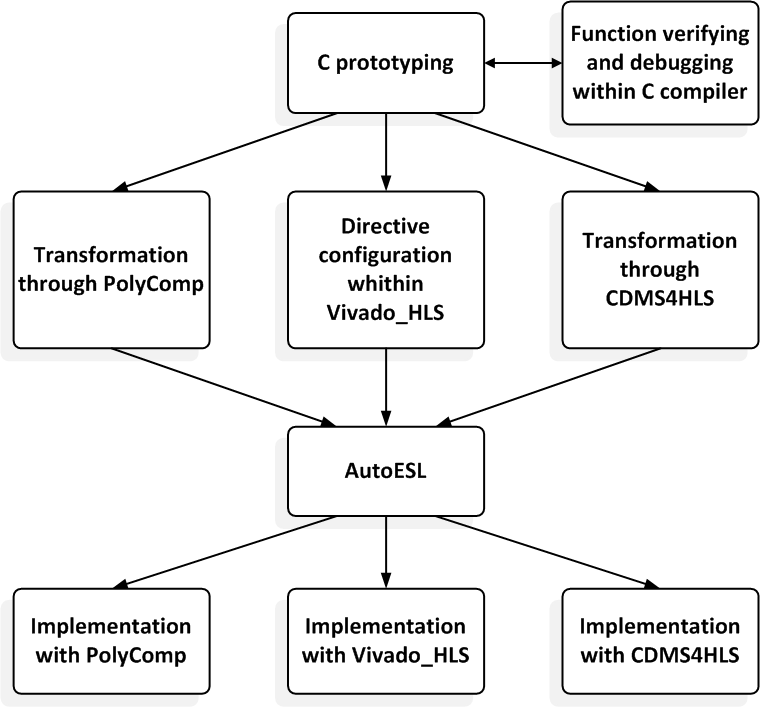
\includegraphics[width=0.8\linewidth]{Experiments.png}\\
    \caption{Implementing flow with different code optimization methods, including PolyComp, manual directive configuration within Vivado\_HLS and CDMS4HLS.}
    \label{Experiments}
    \end{figure}

    \begin{figure}
    \centering
    % Requires \usepackage{graphicx}
    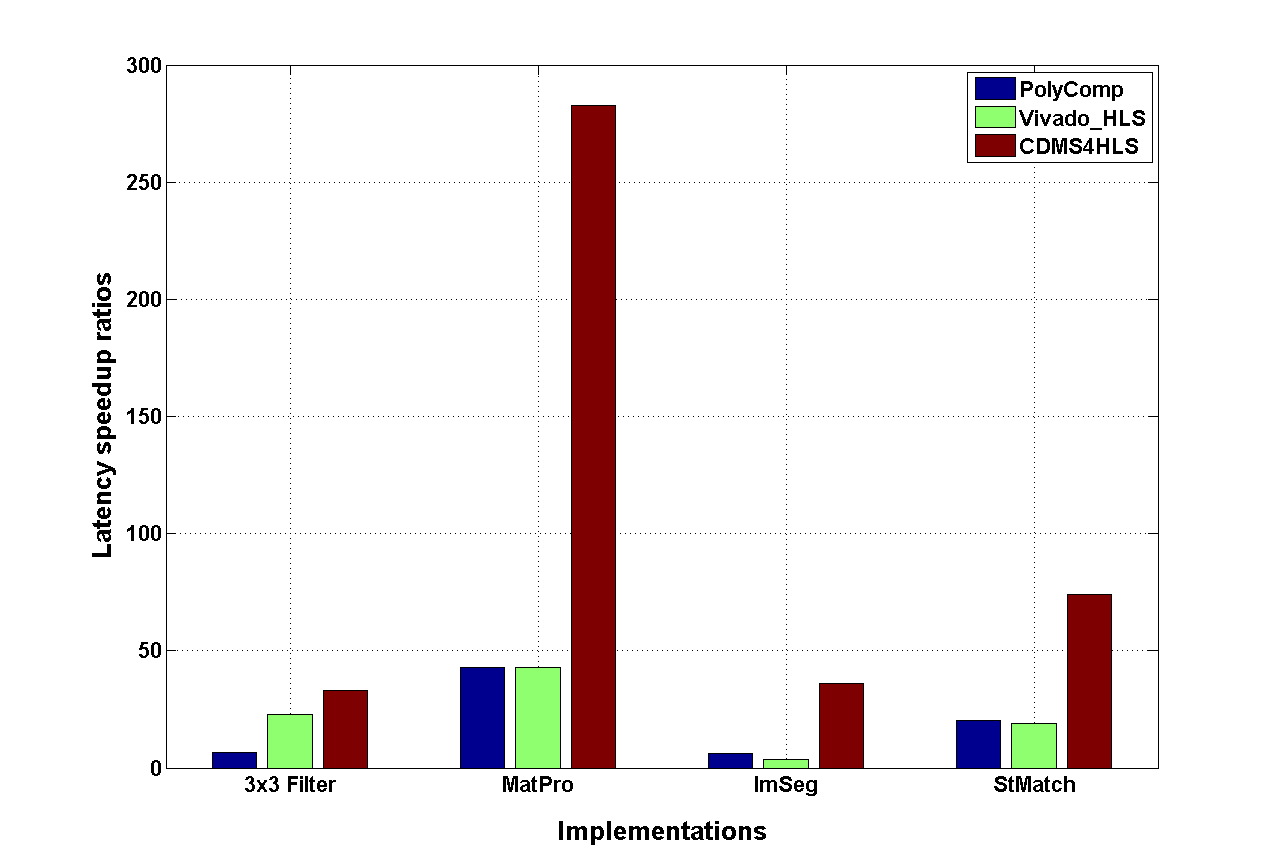
\includegraphics[width=\linewidth]{LatencySpeedupComparison.png}\\
    \caption{Latency speedup comparison.}
    \label{LatencySpeedupComparison}
    \end{figure}
We compare the proposed approach with other two functionally similar design flows (see Fig.\ref{Experiments}) using the source code of four basic image processing algorithms, including $3\times 3$ filter for RGB images, matrix product (MatPro), Image Segmentation using Sobel operator (ImSeg) and Stereo Matching using sum of squared difference (StMatch). We base the first design flow on two improved conventional source-to-source C/C++ compilers: an improved PoCC polyhedral framework \cite{54,65,66} and the Generic Compiler Suite (GeCoS) \cite{55,56,57} (defined as PolyComp), while the other one on the Vivado\_HLS Design Suite \cite{61} (defined as Vivado\_HLS). In order to obtain an unbiased conclusion, all the source codes are synthesized using AutoESL and their data formats are normalized to 32-bit integer numbers. Considering that PolyComp does not have the ability of I/O interface manipulation, we set the I/O protocol of the target implementations as the default of the HLS tool used.

The latency speedups of the three design flows with different algorithms are compared in Fig.\ref{LatencySpeedupComparison}. This result is normalized to the int\_32 original versions of the related algorithms. These three approaches respectively achieve an average of $19.01\times$, $22.19\times$ and $106.54\times$ speedups. This demonstrates that the proposed approach can gain more performance improvements in terms of latency consumption. Compared with the other designs, CDMS4HLS has the ability to manipulate the source code in a lower instructions level, which provide more optimization opportunities to HLS tools. Furthermore, our method can effectively reduce the transition number of the FSM behaviours of the target implementations. For example, the transition number of the MatPro optimized by CDMS4HLS is only half as many as PolyComp and Vivado\_HLS respectively. In additional, it should note that the acceleration gains due to the interface expending are not taken into account. That is, CDMS4HLS and Vivado\_HLS may achieve more speedups than PolyComp.

\section{Conclusion}
\label{sect:conclusion}

This paper presents a novel source-to-source compilation strategy for High-Level Synthesis. Unlike the other studies, the features of HLS procedure and its existing tools are studied in detail. Basing on these efforts, we designed a customized
code and directive manipulation strategy (CDMS4HLS) for it.

The proposed approach improves the performances of the desired designs in various ways, including function and loop hierarchy optimization, symbolic expression manipulation and memory/interface protocol manipulation. In the experiments, we evaluate our approach using four basic algorithms and compare it with two other similar design flows: PolyComp and Vivado HLS. The results demonstrate that CDMS4HLS is an effective code optimization strategy which improves substantially the HLS based FPGA designs.

For the future work, we plan to apply the FPGA design flow improved by the proposed method into some complex real-time image processing applications. Since computationally intensive algorithm may result in a complicate control flow and operation scheduling, more efforts are usually required for development and optimization. Testing and verifying CDMS4HLS according to a practical and complex case can further evaluate its feasibility for commercialization. Meanwhile, we hope that the efforts of this paper can bring some enlightenments to the studies for fast FPGA development framework.

% %% Incldue the content without .tex extension
% \acresetall  % reset the acronyms from the abstract
% % include the figures path relative to the master file
\graphicspath{ {./content/intro/figures/} }

\section{Introduction}
\label{sec:intro}  % \label{} allows reference to this section

Malignant melanoma is the deadliest type of skin cancer, accounting for the vast majority of skin cancer deaths~\cite{CancerFactsFigures2014}. 
According to latest reports, melanoma causes over 20,000 deaths annually in Europe~\cite{forsea2012melanoma}. 
In 2014, the American Cancer Society also reported that the number of new diagnosed cases is 76,100 with 9710 estimated deaths~\cite{CancerFactsFigures2014}. 
%Nevertheless, early diagnosis play a key role since that melanoma being the most treatable kind of cancer.
Nevertheless, melanoma is the most treatable kind of cancer if diagnosed early. 

The clinical diagnosis of early stage melanoma is commonly based on the ``ABCDE'' rule~\cite{abbasi2004early}, defined as Asymmetry, irregular Borders, variegated Colours, Diameters greater than \SI{6}{\milli \metre} and Evolving stages over time. 
In addition, the clinical diagnosis of melanoma is performed through visual inspection and deep analysis of the lesion, using clinical imaging techniques such as dermoscopic imaging. 
However, these inspections and analysis are not easy tasks due to challenges such as similarity of the different lesion types (dysplastic and melanoma) and the necessity to perform patient follow-up over years.
Therefore, the research communities have dedicated their efforts to develop computerized lesion analysis algorithms for classification of melanoma lesions. 
However, akin to other medical applications, the percentage of melanoma cases in comparison with benign and dysplatic cases is far less. 
This problem is frequently referred as ``class imbalanced'' problem~\cite{prati2009data} and has been encountered in multiple areas such as telecommunication managements, bioinformatics, fraud detection, and medical diagnosis. 
Imbalanced data substantially compromise the learning process since most of the standard machine learning algorithms expect balanced class distribution or an equal misclassification cost~\cite{he2009learning}.

Medical data are prone to such drawbacks due to the fact that the portion of diseased samples or patients is far lower than healthy cases.
Furthermore, the detection and classification of minority malignant cases are highly essential so that the \ac{se} of developed algorithms needs to be maximized.
Consequently, the problem of imbalanced data is usually addressed by employing different techniques which do not vitiate the topology of the data.
Despite the fact that classification of malignant melanoma has been extensively studied~\cite{rastgoo2015automatic}, up to our knowledge, only two works tackled the issue implied by imbalanced dataset~\cite{barata2013two,celebi2007methodological}.
Barata~\etal generate new synthetic samples by adding a Gaussian noise with fixed parameters to the samples belonging to the minority class~\cite{barata2013two}.
Celebi~\etal over-sampled their dataset using \ac{smote}~\cite{chawla2002smote} to improve the \ac{se} of their algorithm~\cite{celebi2007methodological}.

This paper provides an insight to the specific problem of classification of imbalanced dataset for malenoma. 
To proceed, we review different techniques proposed by the machine learning community and compile a comprehensive quantitative evaluation. The rest of this paper is organized as follows: an overview of the classification framework designed to investigate data balancing techniques is presented in Sect.\,\ref{sec:mm} while these strategies are described in Sect.\,\ref{sec:met}. A quantitative evaluation is discussed in Sect.\,\ref{sec:exp-res} followed by a concluding section.


% Some stuff that emac's colegues use
%%% Local Variables: 

%%% mode: latex
%%% TeX-master: "../../master"
%%% End: 

          % the file wihtout .tex
% % include the figures path relative to the master file
% \graphicspath{ {./content/method/figures/visual_cues/}{./content/method/figures/}}
\graphicspath{ {./content/method/figures/}}

\begin{figure*}[t]
  \centering{
    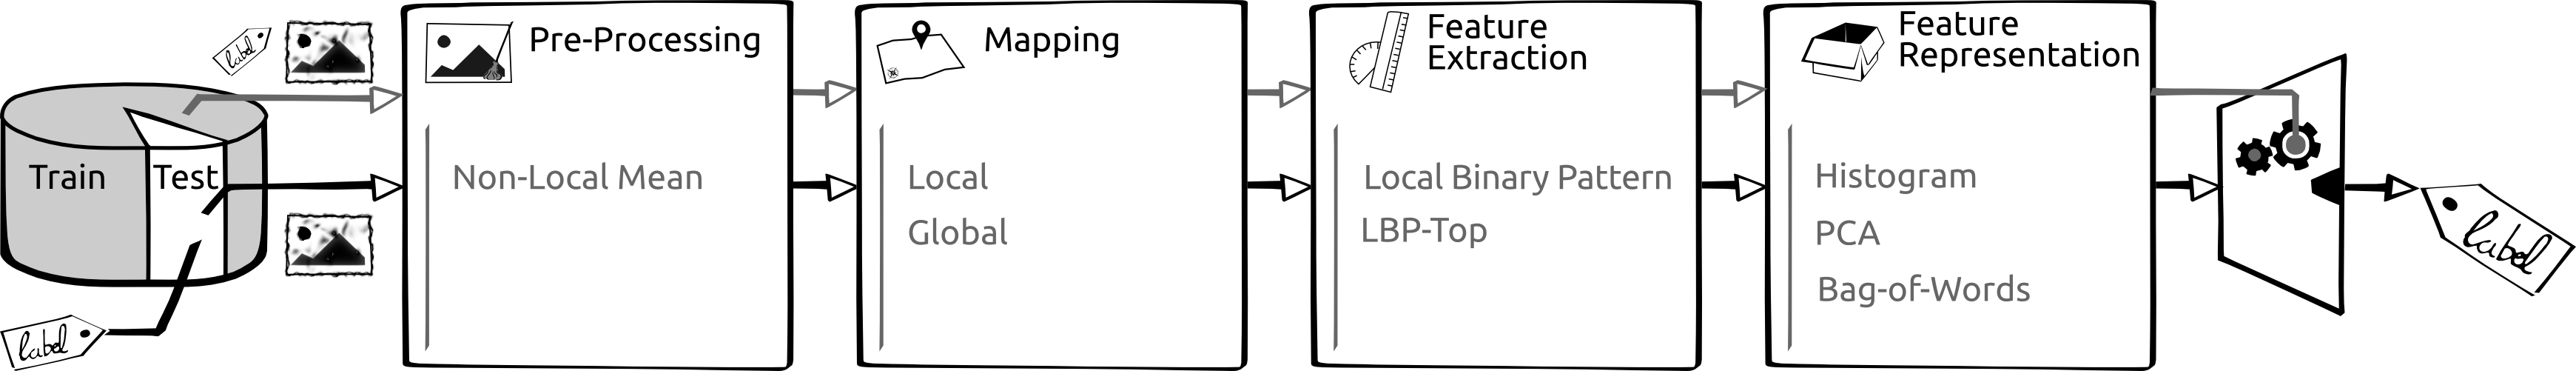
\includegraphics[width=1\textwidth]{ml}}
  \caption{Machine learning classification basic scheme}
  \label{fig:ML-scheme}
\end{figure*}

\section{Materials and Methods}\label{sec:method}

The proposed method, as well as, its experimental set-up for \ac{oct} volume classification are outlined in Fig.\,\ref{fig:ML-scheme}.
The methodology is formulated as a standard classification procedure.
% The available dataset with its acompaining \ac{gt} are divided into training $(S1,l1)$ and testing $(S2,l2)$. 
% The final goal is to represent $S1$ and $S2$ in the feature space $F$ by supplying $(sxF,l1)$ as a training to a classifier, using the trained classifier to estimate $l2$ from $S2xF$ and comparing the estimation with the \ac{gt}.
First, the \ac{oct} volumes are pre-processed as presented in details in Sect.\,\ref{subsec:prepro}.
% This algorithm preserve important details and textures of the original image, while reducing the noise.
The mapping stage is used to determine a discrete set of elements (or structures) which is used for representing the \ac{oct} volume.
Thereafter, two mapping strategies are defined: (i) \emph{global} and (ii) \emph{local} mapping.
In the global mapping approach, a single structure is computed for the image/volume while in the local mapping, a set of structures is defined by sliding a window through the image/volume.
Then, a descriptor is computed for each structure.
The feature extraction and representation are presented in depth in Sect.\,\ref{subsec:feaext} and Sect.\,\ref{subsec:fearep}.
% The feature detection stage correspond to measurements done in $G(Z)$ used for representing $s$ in terms of $ZxG$. 
% This mapping and feature detection steps can be found as a single-steps in the literature.
% The feature extraction procedure combines the elements in $Z$ and its measurements $G(Z)$ to create the final feature space $F$ and project $s$ on it.
A \ac{rf} classifier has been selected to perform the classification of the \ac{oct} volume~\cite{breiman2001random}.
% The design choices are all illustrated in Fig.\,\ref{fig:ML-scheme} and discussed further in this section. The work here presented does not discuss in detail neither the mapping, nor the adopted classifier, further than this lines.
% As a possible mappings, for representing the volumes, 2D image slices of the volume and \color{red}{7x7x7}\color{black} sliding volumes, have been considered. 
% As a classifier, a \color{red}{Random Forest}\color{black} using 100 trees, has been considered.

% \subsection{Data}
% \color{red}{
%   \begin{itemize}
%   \item cross-validation
%   \item our dataset
%   \item DUC dataset
%   \end{itemize}}\color{black}

% For evaluation purposes, the results have been cross-validated, by splitting the data in training and testing using a \ac{lopo} strategy. In this manner for each round a pair \color{red}{dce,normal} has been selected to be used as the round test set, while the rest of the dataset has been used as a training. \color{red}{Doing the cross validation in this manner, has the limitation that despite the fact that the results are robust due to the cross validation, no results variance can be reported. However, and despite this limitation, \ac{lopo} has been choose due to the reduced amount of \ac{oct} volumes available.}\color{black}

% \color{red}{The dataset blablablabal...}\color{black}
% \color{red}{The duc dataset blabla bla...}\color{black}

\subsection{Image pre-processing}\label{subsec:prepro}

\Ac{oct} images are known to be affected by a speckle noise~\cite{schmitt1999speckle}.
Subsequently, \ac{nlm}~\cite{buades2005non} filtering has been successfully used in \ac{us} images to filter similar noise~\cite{Coupe2009} and is used in our framework to denoise each B-scan (i.e. each $x-z$ slice) of the \ac{oct} volumes (see in Fig.\,\ref{subfig:vol}).
%The pre-processing stage in the proposed methodology applies an image denoising method to reduce the speckle noise in \ac{oct} images.
%Since image details and texture of the original image are needed by the following stages in the method, \ac{nlm} algorithm \cite{buades2005non} is used. 
\ac{nlm} filtering offers the advantage to use all the possible self-predictions that the image can provide rather than local or frequency filters such as Gaussian, anisotropic or Wiener filters~\cite{buades2005non}.
An example of filtering using \ac{nlm} filter on \ac{oct} image is depicted in Fig\,\ref{subfig:raw} and Fig.\,\ref{subfig:nlm}.

\begin{figure*}[t]
  \centering
  \hspace*{\fill}
  \subfloat[][]{\label{subfig:vol}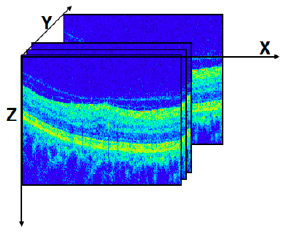
\includegraphics[width=0.3\linewidth]{volume.png}} \hfill
  \subfloat[][]{\label{subfig:raw}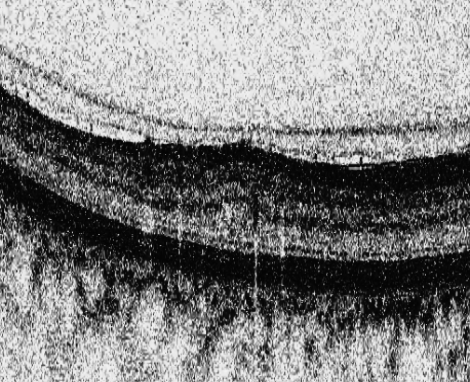
\includegraphics[width=0.3\linewidth]{raw_crop_grey.png}} \hfill
  \subfloat[][]{\label{subfig:nlm}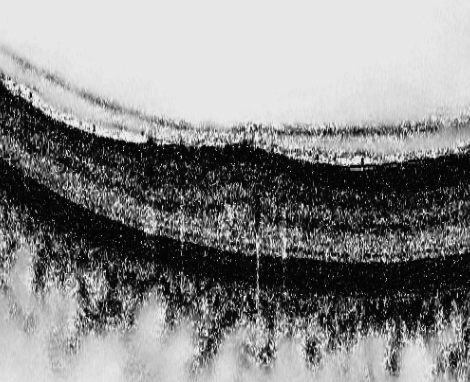
\includegraphics[width=0.3\linewidth]{nlm_crop_grey.png}}
  \hspace*{\fill}
  \caption{\ac{oct}: (a) Organization of the \ac{oct} data - (b) Original image - (c) \ac{nlm} filtering.}
  \label{fig:denoise}
\end{figure*}

\subsection{Features extraction}\label{subsec:feaext}

\ac{lbp} is a texture descriptor based on the signs of the differences of a central pixel with respect to its neighboring pixels~\cite{ojala2002multiresolution}. 
%More precisely, this descriptor encodes the intensity differences of a central pixel ($g_c$) with its neighboring pixels ($g_{p}$), within in a defined neighborhood of radius $R$. 
These differences are encoded in terms of binary patterns as in~Eq.\,\eqref{Eq:LBP}: 

\begin{equation}\label{Eq:LBP}\footnotesize
LBP_{P,R} = \sum_{p=0}^{P-1}s(g_{p} - g_{c})2^{p} \ , \  s(\cdot) = \begin{cases}
    1  & \ \text{if } (g_{p} - g_{c}) \geq 0\\
    0  & \ \text{otherwise}\\
  \end{cases} \ ,
\end{equation}

% \begin{align} \label{Eq:LBP}
% LBP_{P,R} = \sum_{p=0}^{P-1}s(g_{p} - g_{c})2^{p}& \ , \\
% \text{where } &s(\cdot) = \begin{cases}
%     1  & \quad \text{if } g_{p} - g_{c} \geq 0\\
%     0  & \quad \text{otherwise}\nonumber\\
%   \end{cases} \ .
% \end{align}
\noindent where $g_c$, $g_{p}$ are the intensities of the central pixel and a given neighbor pixel, respectively. $P$ is the number of sampling points in the circle of radius $R$. Figure~\ref{subfig:lbp} illustrates the meaning of $P$ and $R$.

Ojala\,\textit{et al.} further extend the original \ac{lbp} formulation to achieve rotation invariance at the expense of limiting the texture description to the notion of circular ``uniformity''~\cite{ojala2002multiresolution}. Volume encoding is later proposed by Zhao\,\textit{et al.} by computing \ac{lbp} descriptors in each orthogonal planes, so called \ac{lbptop}~\cite{zhao2012rotation}.

\begin{figure*}[t]
  \centering
  \hspace*{\fill}
  \subfloat[][]{\label{subfig:lbp}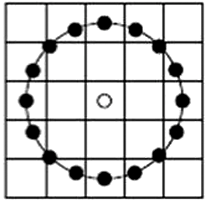
\includegraphics[height=0.1\textheight]{lbp.png}} \hfill
  \subfloat[][]{\label{subfig:lbptop}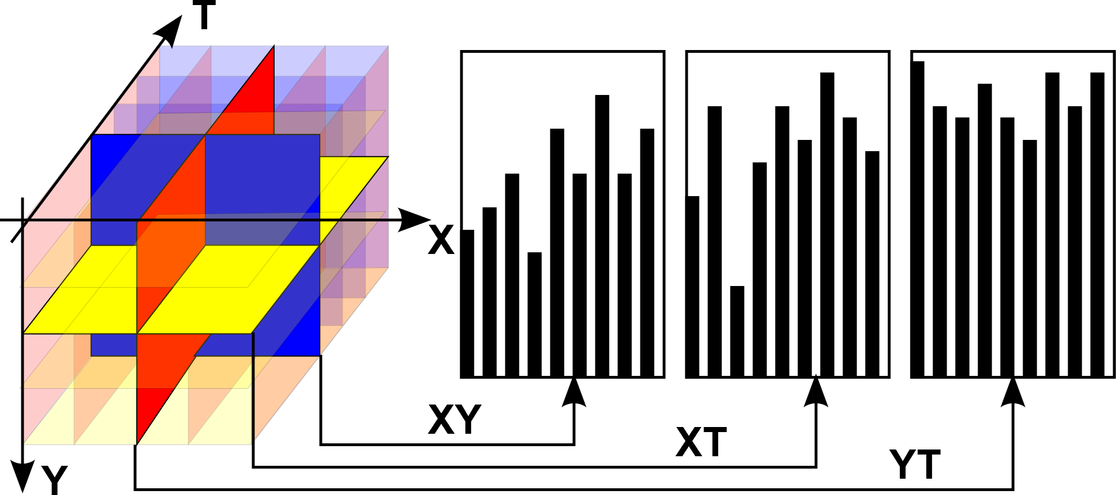
\includegraphics[height=0.1\textheight]{LBPTOP_fig.png}}
  \hspace*{\fill}
  \caption{The different \ac{lbp} descriptors: (a) \ac{lbp} with $(R=2,P=16)$ - (b) \ac{lbptop}~\cite{zhao2012rotation}.}
  \label{fig:lbp}
\end{figure*}

\subsection{Feature representation}\label{subsec:fearep}

Each \ac{oct} volume can be described by its texture and we employed two strategies.

\begin{description}

\item[Low-level representation] The texture descriptor of an \ac{oct} volume is defined as the concatenation of the \ac{lbp} histograms. Regarding the \ac{lbptop}, the feature descriptor is computed through the concatenation of the \ac{lbp} histograms of the three orthogonal planes. 
Furthermore, the size of this entire feature vector is defined according to the mapping strategy chosen (see Fig.\,\ref{fig:ML-scheme}).

\item[High-level representation] According to the chosen mapping strategy, the low-level representation can lead to a high dimensional feature space. 
High-level representation simplifies this high dimensional feature space into a more discriminant lower space. 
\Ac{pca} and \ac{bow} among other methods, are used for this purpose~\cite{Sivic2003}. 
Although \ac{pca} maps the data according to their variance, \ac{bow} models represent the features by creating a visual dictionary, or ``codebook'', from the set of low-level features.
The set of low-level features is clustered using \textit{k}-means to create the codebook with \textit{k} defining the number of visual words.
After creating the codebook, each of the training example is represented as a histogram of size \textit{k} obtained by calculating the frequency of occurrences of each of the \textit{k} words in the features extracted from the training example. 

\end{description}

%\subsubsection{Low-level features} are extracted considering the whole volume using LBP and 3D-LBP descriptors. 
% LBP is a discriminative rotation invariant feature descriptor proposed by Ojala et al. \cite{ojala2002multiresolution}. 
% LBP descriptor encodes the intensity differences of a central pixel ($g_c$) with its neighboring pixels ($g_{p}$), within in a defined neighborhood of radius $R$. The differences are encoded in terms of binary patterns as in~Eq. \ref{Eq:LBP}: 

% \begin{equation} \label{Eq:LBP}
% LBP_{P,R} = \sum_{p=0}^{P-1}s(g_{p} - g_{c})2^{p},
% \end{equation}
% where $s(a) = 1$ if $a \geq 0$, and $s(a)=0$ otherwise. $P$ is the number of sampling points in the circle of radius $R$.

% The binary patterns are calculated for each pixel in the given image and their histogram defines the final descriptor.
% The LBP histograms are computed for each slice of the volume and are concatenated into a single histogram. This forms the first low-level feature.
% The second low-level descriptor is defined in a similar manner as the first one. However principal component analysis (PCA) is applied to the concatenated histograms in order to reduce the dimension.

% For the third low-level descriptor, since the OCT data is a 3D volume, following the approach of Zhao \textit{et al}. \cite{zhao2007dynamic}, we extract 3D-LBP by considering three orthogonal planes, XY, XZ and YZ. Note that $X$, $Y$, and $Z$ are respectively the horizontal, vertical and depth direction of the OCT volume as shown in Figure~\ref{fig:oct_data}(a).
% LBP patterns are computed for each of the three planes, and the obtained three histograms are concatenated into a final 3D-LBP descriptor.



% \subsubsection{High-level features} - are extracted using bag of words (BoW) approach which is a feature representation technique based of creating a visual dictionary, or codebook, from a set of low-level features~\cite{Sivic2003}. 
% To do so, the OCT images are divided into local patches and LBP histograms are computed for every local patch.
% This set of LBP histograms is then used to create a codebook using K-means clustering. If we define $K$ clusters in the feature space, then the visual dictionary will contain $K$ words each one being the center of one cluster.
% After creating the codebook, each of the training example is represented as a histogram of size $K$ obtained by calculating the frequency of occurrences of each of the $K$ words in the features extracted from the training example. 
% Note that in the 2D case, each slice is divided into patches of size $N\times N$ and we extract 2D-LBP from each patch, while in the 3D case, the volume is divided into $N \times N \times N$ patches and 3D-LBP histograms are computed. In our experiments in Section 3, we set $N=7$, and vary the size of the codebook $K$ in the range $\{2, 4, 8, 16, 32, 64, 100 \}$.
% % \tikzstyle{block} = [rectangle, draw, fill=gray!20, text = black,
    text width=6em, text centered, rounded corners, minimum height=4em , minimum width = 6em]
    % \tikzstyle{line} = [draw, -latex']
  \tikzstyle{myarrow}=[->, thick]
    \tikzstyle{line}=[-, thick]
    \tikzstyle{block2} = [rectangle, draw, fill=white!20,
    text width=6em, text centered, rounded corners, minimum height=4em, minimum width = 6em]
    \tikzstyle{block3} = [rectangle, draw, fill=gray!20, text = black,
    text width=7em, text centered, rounded corners, minimum height=4em , minimum width = 7em]
\def\blockdist{1}
\def\edgedist{1.5}
  %%%% The Framework Sparse Coding 

\begin{figure*}
 \begin{center}
   \begin{tikzpicture}[node distance = 1cm,scale=0.6, every node/.style={scale=0.6}]
%(FEx.east|- FEx.south)
    \node [block2] (input) {Training image};
    %\node [block, right of = input, node distance = 2.8cm](Seg){Segmentation}; 
    \node [block, right of=input,node distance = 2.8cm](De){Denoising};
    \node [block, right of=De,node distance = 2.8cm](FEx){Feature extraction};
    \path (FEx.east)+(+0.8,0) node (g) {};
    
    %%% Sparse Coding Block
    \node [block3, right of=g,node distance = 1.7cm](DL){Dictionary learning /k-means};
    \node [block3, below of=DL,node distance = 2.5cm](PR){Projection};
    \begin{pgfonlayer}{background}
      \path (DL.west |- DL.north)+(-0.4,-0.1+\blockdist) node (a) {};
      \path (PR.east |- PR.south)+(+0.4,-0.7) node (b) {};          
      \path[fill=gray!10,rounded corners, draw=gray!20, dashed] (a) rectangle (b);
    \end{pgfonlayer}
\path (DL.west |- DL.north)+(+1.2,-0.5+\blockdist) node (SP) {\textbf{Bag of Features}};
\path (PR.east |- PR.south)+(-1.3,-0.4+\blockdist) node (c){};
\path (PR.east)+(-3.15,0) node (d) {};

%%% Testing 
\node [block, below of=FEx, node distance = 2.5cm](FE2){Feature extraction};
\node [block, below of=De, node distance = 2.5cm](De2){Denoising};
% \node [block, below of=Seg, node distance = 2.5cm](Seg2){Segmentation}; 
\node [block2, below of=input, node distance = 2.5cm](TestImg){Testing image};

%%% 
\node [block, right of=PR, node distance = 3.6cm](Pool){Visual words histogram};
\path (Pool.east) + (0.3,0) node (f){}; 
\path (Pool.east) + (0.2,-0.1) node (f1){}; 

%%% Classification
\node [block, right of = Pool, node distance = 3.5cm] (Pre){Prediction}; 
    \node [block, above of = Pre, node distance = 2.5cm] (Learn){Learning}; 
    \begin{pgfonlayer}{background}
      \path (Learn.west |- Learn.north)+(-0.4,-0.1+\blockdist) node (h) {};
    \path (Pre.east |- Pre.south)+(+0.4,-0.7) node (i) {};          
    \path[fill=gray!10,rounded corners, draw=gray!20, dashed] (h) rectangle (i);
\end{pgfonlayer}
\path (Learn.west |- Learn.north)+(+1.1,-0.5+\blockdist) node (Clas) {\textbf{Classification}};
\path (Pre.east |- Pre.south)+(-1.3,-0.4+\blockdist) node (j){};
\path (f1.north)+(0, 2.5) node (k) {};
\path (Pre.east) + (1.2,0) node (k1) {P(..)}; 

    % Draw edges
    \draw [line] (input) -- (De) -- (FEx); 
    \draw [myarrow] (FEx)-- (DL);
    \draw [myarrow] (DL) -- (PR) ; 
    \draw [line] (TestImg) -- (De2) -- (FE2); 
    \draw [myarrow] (FE2) -- (PR) ;
    \draw [line] (PR) -- (Pool); 
    \draw [myarrow] (Pool) -- (Pre); 
    \draw [line] (f1.north) -- + (0,2.5)(k.south); 
    \draw [myarrow] (k.south)+ (0,0.1)  -- (Learn.west); 
    \draw [myarrow] (Pre) -- (k1);

    \end{tikzpicture}
    \end{center}
    

\caption{Bag of features framework} 
\label{fig:BoF-framework}

\end{figure*}

% \subsection{Classification}

% Random Forest is an ensemble of decision trees and was introduced by~\cite{breiman2001random}.
% The ensemble uses each tree to predict an output and finalize the ultimate prediction by aggregating the outputs of all tress. 
% This classifier learns the data by training multiple decision trees on bootstrap samples of the original data. 
% Each bootstrap of D dimension is used for training one decision tree and at each node, the best split among randomly ($d << D$) selected subset of descriptors is chosen. 
% Each tree is grown to its maximum length without any pruning. 
% In the prediction stage a sample is voted by each tree and it is labeled by considering the majority of the votes.


%%% Local Variables: 
%%% mode: latex
%%% TeX-master: "../../master"
%%% End: 
 
% % % include the figures path relative to the master file
% \graphicspath{ {./content/results/figures/} }

\section{Experiments and Validation}\label{sec:exp}

\subsection{Datasets}

In this work, we validated our classification framework using two different datasets.

\begin{description}

\item[SERI]- datasets were acquired by Singapore Eye Research Institute (SERI), using CIRRUS TM (Carl Zeiss Meditec, Inc., Dublin, CA) \ac{sdoct} device. The datasets consist of 32 \ac{oct} volumes (16 \ac{dme} and 16 normal cases). Each volume contains 128 B-sane with  dimension of 512 $\times$ 1024 pixels.  All \ac{sdoct} images are read and assessed by trained graders and identifies as normal or \ac{dme} cases based on evaluation of retinal thickening, hard exudates, intraretinal cystoid space formation and subretinal fluid.

\item[Duke] - datasets published by Srinivasan et al. \cite{Srinivasan2014} were acquired in Institutional Review Board-approved protocols using Spectralis \ac{sdoct} (Heidelberg Engineering Inc., Heidelberg, Germany) imaging at Duke University, Harvard University and the University of Michigan. This datasets consist of 45 \ac{oct} volumes (15 \ac{amd}, 15 \ac{dme} and 15 normal). In this study we only consider a subset of the original data containing 15 \ac{dme} and 15 normal \ac{oct} volumes.

\end{description}

\begin{tiny}
  \begin{table*}[b]
\caption{Obtained results using SERI datasets.}% using \ac{rf} with 100 trees. High-level features with \ac{bow} are obtained with $K$ = 32 visual-words.}
\centering
\begin{tabular}{lcclcclcccclcclcccclcclc}
\toprule
Features 	& & &\multicolumn{4}{c}{$8^{riu2}$}&	 & & & &\multicolumn{4}{c}{$16^{riu2}$}& & & & &\multicolumn{4}{c}{$24^{riu2}$} &\\
  \cmidrule(l){2-8}  \cmidrule(l){10-16}  \cmidrule(l){18-24}
	       & & & SE & & & SP & & & & & SE & & & SP & & & & & SE & & & SP & \\
\midrule
  	\ac{lbp}					& & & 43.75 & & & 43.75 & & & & & 37.50 & & & 50.00 & & & & & 50.00 & & & 62.50 & \\
 	\ac{lbptop}				& & & 56.25 & & & 62.50 & & & & & \textbf{87.50} & & & \textbf{75.00} & & & & & 68.75 & & & 68.75 & \\
	\ac{lbp}+\ac{pca}		& & & 50.00 & & & 62.50 & & & & & 56.25 & & & 37.50 & & & & & 68.75 & & & 68.75 & \\
	\ac{lbp}+\ac{bow}		& & & 50.00 & & & 81.25 & & & & & 57.50 & & & 68.75 & & & & & 50.00 & & & 50.00 & \\
	\ac{lbp}+\ac{bow}+\acs{sw}		& & & 75.00 & & & 87.50 & & & & & \textbf{81.25} & & & \textbf{75.00} & & & & & 68.75 & & & 62.5 & \\
	\ac{lbptop}+\ac{bow}+\acs{sw}		& & & 62.50 & & & 68.75 & & & & & 56.25 & & & 37.50 & & & & & 37.50 & & & 43.75 & \\
\bottomrule
\end{tabular}
\label{tab:SERI-data}
\end{table*}
\end{tiny}

\begin{tiny}
  \begin{table*}[t]
\caption{Obtained results using Duke datasets.}% using \ac{rf} with 100 trees. High-level features with \ac{bow} are obtained with $K$ = 32 visual-words.}
\centering
\begin{tabular}{lcclcclcccclcclcccclcclc}
\toprule
Features 	& & &\multicolumn{4}{c}{$8^{riu2}$}&	 & & & &\multicolumn{4}{c}{$16^{riu2}$}& & & & &\multicolumn{4}{c}{$24^{riu2}$} &\\
  \cmidrule(l){2-8}  \cmidrule(l){10-16}  \cmidrule(l){18-24}
	       & & & SE & & & SP & & & & & SE & & & SP & & & & & SE & & & SP & \\
\midrule
 	\ac{lbptop}				& & & 80.00& & & 93.33 & & & & & 73.33 & & & 86.67 & & & & & 73.33 & & & 86.67 & \\
	\ac{lbp}+\ac{bow}+\acs{sw}		& & & 80.00 & & & 86.67 & & & & & 86.67 & & & 100 & & & & &93.33 & & & 86.67 & \\
	\ac{lbptop}+\ac{bow}+\acs{sw}		& & & 80.00 & & & 86.67 & & & & & 86.67 & & & 86.67 & & & & & 60.00 & & & 80.00 & \\
\bottomrule
\end{tabular}
\label{tab:Duke-data}
\end{table*}
\end{tiny}

\begin{tiny}
\begin{table*}[t]
\caption{Comparing the proposed method by \cite{Venhuizen2015} on SERI and Duke datasets.}% with the \textbf{our two} best proposed methods. $K$ = 32 and \ac{rf} is trained using 100 tress}
\centering
\begin{tabular}{lcclcclcccclcclc}
\toprule
Data sets 	& & &\multicolumn{4}{c}{SERI}& & & & &\multicolumn{4}{c}{Duke} & \\
  \cmidrule(l){2-8}  \cmidrule(l){10-16}
	         & & & SE & & & SP & & & & & SE & & & SP & \\
\midrule
Venhuizen~\textit{et al.} \cite{Venhuizen2015} 		& & & 61.53 & & & 58.82 & & & & & 71.42 & & & 68.75 & \\
\{\ac{lbp}+\ac{bow}+\ac{sw}\},$16^{riu2}$ 	& & & 81.25 & & & 75.00 & & & & & 86.67 & & & 100.00 &  \\
\{\ac{lbptop}\},$16^{riu2}$				& & & 87.50 & & & 75.00 & & & & & 73.33 & & & 86.76 &  \\


\bottomrule
\end{tabular}
\label{tab:ComparisonRefandOurs}
\end{table*}

\end{tiny}

\subsection{Experiments \& Results}

Both datasets are filtered to attenuate the effect of speckle noise.
SIRE dataset is processed using \ac{nlm} as stated in Sect.\,\ref{subsec:prepro}.
The different parameters were empirically tested and fixed such that the patch size, the search window and the filtering parameter were set to $(15 \times 15)$, $(35 \times 35)$ and $0.4$, respectively.
However, Duke dataset is already filtered using BM3D method~\cite{Srinivasan2014}.
For both datasets, \ac{lbp} and \ac{lbptop} features are extracted for different sampling points of 8, 16 and 24 for radius of 1, 2 and 3, respectively.
Two different mapping strategies are used: (i) \emph{global} mapping corresponding to the 2D B-scan for \ac{lbp} or the 3D volume for \ac{lbptop} and (ii) \emph{local} mapping considering to a set of 2D \ac{sw} of size $(7 \times 7)$ for \ac{lbp} or the 3D sub-volume for \ac{lbptop} of size $(7 \times 7 \times 7)$.
For the high-level representation, when \ac{pca} is applied, the eigenvectors associated with the largest $99\%$ cumulative eigenvalues are selected to reduce the number of dimensions. In \ac{bow} approach, an empirical search was performed to find the optimal number of visual words which is finally fixed to 32.
The number of trees for each \ac{rf} classifier was fixed to 100.

For evaluation purposes, all the results are expressed in terms of \ac{se} and \ac{sp} using a \ac{lopocv} strategy.
Thus, at each round a pair \ac{dme}-normal volume is selected for testing while the rest are used for training.
The use of \ac{lopocv} implies that no variance in \ac{se} and \ac{sp} can be reported.
However, and despite this limitation, \ac{lopocv} has been employed due to the small size of the datasets. 
%Performing \ac{lopo} cross validation has the limitation that despite achieving robust results due to the cross validation, no variance in \ac{se} or \ac{sp}, can be reported.
%For evaluation purposes, the results are cross-validated, by splitting the data in training and testing using a \ac{lopo} strategy. 
%In this manner for each round a pair of \ac{dme} and normal \ac{oct} volume is selected to be used as the round test set, while the rest of the datasets are used for training. 
%Performing \ac{lopo} cross validation has the limitation that despite achieving results are robust due to the cross validation, no variance in results can be reported. 
%The classification performances are reported in terms of \ac{se} and specificity \ac{sp}.
%A larger testing set can not be used here, due to the limited amount of available \ac{oct} volumes.

\begin{description}

\item[Experiment \#1] is carried out on SERI dataset. Both low and high level feature representation are extracted and tested. The results are reported in Table~\ref{tab:SERI-data}.

\item[Experiment \#2] is carried out on the Duke dataset~\cite{Srinivasan2014}. The \ac{oct} volumes provided by this dataset are cropped, with different sizes.
Subsequently, the experiments involving the mapping using 2D B-scan do not comply with these requirements and thus are not carried out.
The obtained results for this experiment are shown in Table~\ref{tab:Duke-data}.

\item[Experiment \#3] presents a comparison of our best approaches with the method reported in~\cite{Venhuizen2015} in-house implemented and are expressed in Table~\ref{tab:ComparisonRefandOurs}.

\end{description}
% The SERI datasets are provided in complete \ac{oct} volumes by 512$\times$1024$\times$128 dimensions. Using this datasets, first the three low-level features such as \ac{lbp}, \ac{lbp}+\ac{pca} and \ac{lbptop} are extracted. The rotation invariant uniform ($riu2$) descriptors are calculated with the $P$ number of 8, 16 and 24 for the radius if 1, 2 and 3 respectively. The features are classified using RF with 100 tress. Table \ref{tab:LbPTopVolumeResult} shows the relative results for $8riu2$, $16riu2$, $24riu2$ and their combination $8riu2 + 16riu2 + 24riu2$. The results are presented in terms of \ac{se} and \ac{sp} percentages.

% The second experiment is carried out using high-level features and \ac{bow} approach, on SERI datasets. The first high-level feature \ac{lbp}+\ac{bow} is obtained by applying \ac{bow} with 32 visual-words on the previously low-level \ac{lbp} features (applied on each B-scan). The second and third high-level descriptors are obtained using a dense approach by applying the \ac{sw} of size (7$\times$7) on each B-scan and \ac{sw} of size (7$\times$7$\times$7) to the whole volume respectively. \ac{lbp}+\ac{bow}+\ac{sw} represent the second high-level feature where the 2D-\ac{lbp} features are extracted for each sliding window on each B-scan and the visual-words are selected from the pool, consisting of their histograms. The third high-level feature, \ac{lbptop}+\ac{bow}+\ac{sw}, is defined using \ac{lbptop}. By using the sliding window the 3D-\ac{lbp} features are extracted for each patch. Same as previous experiment with low-level features, the descriptors are calculated with the $P$ number of 8, 16 and 24 for the radius if 1, 2 and 3 respectively. The obtained results of this experiment are illustrated in Tab. \ref{tab:SERIBoWResult}.

% In order to compare our proposed framework the third experiment is carried out using the subsection of Duke datasets \cite{Srinivasan2014}. The OCT volumes provided by this datasets are of different volume size, cropped and denoised by the method of authors choice. Subsequently only the second experiment with high-level features and low-level \ac{lbptop} features comply with these requirements. The number of visual-words and the size of \ac{sw} for 2D and 3D features are the same than the previous experiment. The 2D and 3D \ac{lbp} features are extracted with $P$ number of 8, 16 and 24 for the radius if 1, 2 and 3 respectively. The obtained results for this experiment are shown in Tab. \ref{tab:DukeBoWResult}.
%----------

%%% Local Variables:
%%% mode: latex
%%% TeX-master: "../../master"
%%% End:

% %% include the figures path relative to the master file
\graphicspath{ {./content/results/figures/} }
\definecolor{acm}{rgb}{0.8 0.7254901960784313 0.4549019607843137}
\newcommand{\acmColor}{yellow}

\definecolor{ml}{rgb}
{0.3333333333333333  0.6588235294117647 0.40784313725490196}
\newcommand{\mlColor}{green}

\definecolor{other}{rgb}
{0.5058823529411764  0.4470588235294118 0.6980392156862745}
\newcommand{\otherColor}{purple}

\definecolor{db}{rgb}
{0.7686274509803922  0.3058823529411765 0.3215686274509804}
\newcommand{\dbColor}{red}

\definecolor{aov}{rgb}
{0.2980392156862745  0.4470588235294118 0.6901960784313725}
\newcommand{\aovColor}{blue}

\tikzstyle{acmStyle} = [fill=acm]
\tikzstyle{mlStyle} = [fill=ml]
\tikzstyle{otherStyle} = [fill=other]
\tikzstyle{nodeBase} = [ rectangle,rounded corners=2pt]




\begin{figure*}[!htb]
  \centering

  \begin{tikzpicture}
  \tikzstyle{noMargin} = [inner sep=0mm, outer sep=0mm]
  \node[noMargin](a){
    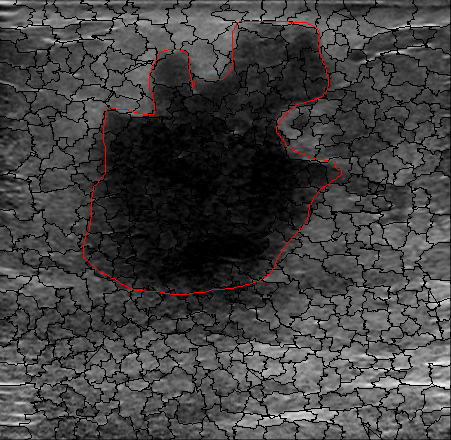
\includegraphics[trim= 20 0 30 0, clip, height=3cm]{goodQSorigin}
  };
  \node[noMargin, right= 3pt of a](b){
    
\includegraphics[trim= 20 0 30 0, clip, height=3cm]{goodQSseg}
    };
  \node[noMargin, right= 3pt of b](c){
    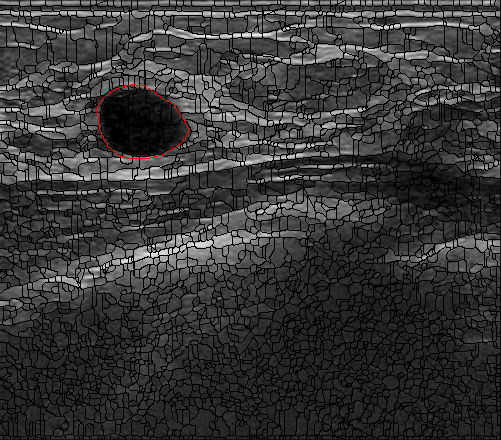
\includegraphics[trim = 0 90 0 0, clip, height=3cm]{fporigin}
  };
  \node[noMargin, right= 3pt of c]{
    \begin{tikzpicture}
      \node[noMargin](d){
      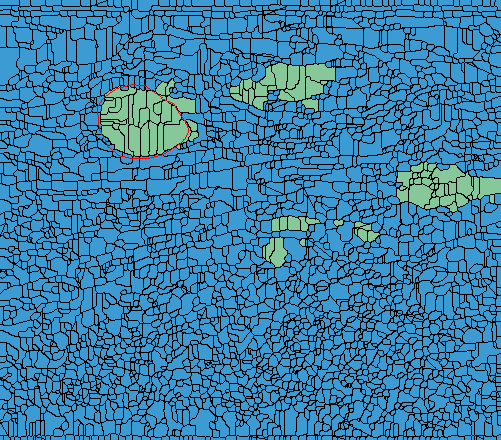
\includegraphics[trim = 0 90 0 0, clip, height=1.2cm]{fpnohom}
      };
      \node[noMargin, below= 5pt of d]{
      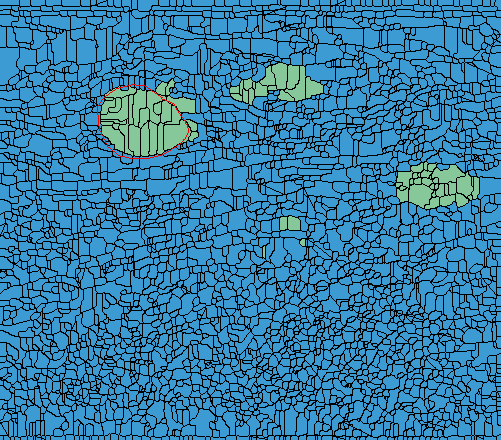
\includegraphics[trim = 0 90 0 0, clip, height=1.2cm]{fpHom}
      };
    \end{tikzpicture}
  };

  \end{tikzpicture}

  \caption{\footnotesize Qualitative results.
    (a) Example 1: orignal image, super-pixels' delineations and \ac{gt}.
    (b) Differences between \ac{gt} and the delination resulting from super-pixels' boundary.
    (c) Ex. 2.
    (d) weak $V(\cdot,\cdot)$
    (e) strong $V(\cdot,\cdot)$
    \vspace{-10pt}
    }
  \label{fig:results}
\end{figure*}


\section{Method evaluation and comparison}

\begin{figure*}[!htb]
\centering
  \begin{subfloat}
    {\tiny 
\newcommand{\myCoord}[1]{
  \tikz[remember picture]{\coordinate[remember picture] (#1) at (0,0);
    %\fill[red] (#1) circle[radius=1pt];
  }
}

\newcommand{\drawBox}[5] {
  % draw a colored bar [0..MaxValue] 
  % parameters:
  %  #1 - bar color
  %  #2 - bar width
  %  #3 - bar height
  %  #4 - MaxValue
  %  #5 - actual Value
  \begin{tikzpicture}[baseline=(value.center)]
    \def\w{#2}                   % width of a box
    \def\h{#3}                   % height of a box
    \pgfmathsetmacro{\v}{#5/#4}  % value to display in ratio [0-1]  
    \pgfmathsetmacro{\V}{100*\v} % value to display in percentage   
    \def\x{\v*\w}                % position of the desired value

    % draw rectangle (value dims between color and: white-body, gray-border)
    \draw[draw=#1!\V!gray!] (0,0) rectangle (\w,\h);
    \filldraw[fill=#1!\V!white!, draw=#1!\V!gray!] (0,0) rectangle (\x,\h);
    % display the value
    \path (0,0) -- (0,\h) node[midway,anchor=west] (value) {#5};

%    \draw [blue] (current bounding box.south west) rectangle (current bounding box.north east);
  \end{tikzpicture}
}

\centering
\begin{tabular}{lcccccccccccccccc}
  Method Id:%\textsuperscript{[ref]}:
              &a%\cite{Liu:2010p14328}
              &b%\cite{Gao:2012p14336}
              &c%\cite{AlemanFlores:2007p14310}
              &d%\cite{Huang:2012p14313}
              &e%\cite{Madabhushi:2003p6036}
              &f%\cite{hao2012combining}
              &g%\cite{Zhang:2010p14317}
              &h%\cite{Xiao:2002p5639}
              &i%\cite{massich2010lesion}
              &j%\cite{Shan:2012p14347}
              &k%\cite{Yeh:2009p11985}
              &l%\cite{Horsch:2001p6028}
              &m%\cite{Gomez:2010p14339}
              &n%\cite{Huang:2005p11636}
              &o%\cite{Huang:2007p6100}
              &p%\cite{Cui:2009p14325}\\
  \\\hline \\
  Dataset size:     & 76   & 20   & 32   & 20   & 42   & 480  & 347    & 352  & 25
                    & 120  & 6    & 400  & 50   & 20   & 118  & 488 \\

  techonlogy used for:  &\\
  \quad detection       & \myCoord{Adetect} & \myCoord{Bdetect} & \myCoord{Cdetect} & \myCoord{Ddetect} & \myCoord{Edetect} 
                        & \myCoord{Fdetect} & \myCoord{Gdetect} & \myCoord{Hdetect} & \myCoord{Idetect} & \myCoord{Jdetect}
                        & \myCoord{Kdetect} & \myCoord{Ldetect} & \myCoord{Mdetect} & \myCoord{Ndetect} & \myCoord{Odetect}
                        & \myCoord{Pdetect}\\

  \quad segmetnation    & \myCoord{Aseg} & \myCoord{Bseg} & \myCoord{Cseg} & \myCoord{Dseg} & \myCoord{Eseg} 
                        & \myCoord{Fseg} & \myCoord{Gseg} & \myCoord{Hseg} & \myCoord{Iseg} & \myCoord{Jseg}
                        & \myCoord{Kseg} & \myCoord{Lseg} & \myCoord{Mseg} & \myCoord{Nseg} & \myCoord{Oseg}
                        & \myCoord{Pseg}\\

  \quad post-processing & \myCoord{App} & \myCoord{Bpp} & \myCoord{Cpp} & \myCoord{Dpp} & \myCoord{Epp} 
                        & \myCoord{Fpp} & \myCoord{Gpp} & \myCoord{Hpp} & \myCoord{Ipp} & \myCoord{Jpp}
                        & \myCoord{Kpp} & \myCoord{Lpp} & \myCoord{Mpp} & \myCoord{Npp} & \myCoord{Opp}
                        & \myCoord{Ppp}\\
  \\\hline \\
  \ac{aov} (in \%): & 88.1 & 86.3 & 88.3 & 85.2 & 62.0 & 75.0 & 84.0   & 54.9 & 64.0
                    & 83.1 & 73.3 & 73.0 & 85.0 & 78.6 & 77.6 & 74.5\\
\end{tabular}


\begin{tikzpicture}[remember picture, overlay]
  % single step ACM
  \foreach \x in {Cseg, Cpp, Dpp, Epp, Npp, Opp, Ppp}
  \node[nodeBase, acmStyle, anchor=center] at (\x) {};

  % single step ML
  \foreach \x in {Edetect, Gdetect, Idetect, Pseg}
  \node[nodeBase, mlStyle, anchor=center] at (\x) {};

  % single step Other
  \foreach \x in {Eseg, Iseg, Ipp, Jpp, Kseg, Lseg, Mseg, Mpp, Nseg}
  \node[nodeBase, otherStyle, anchor=center] at (\x) {};

  \node[nodeBase, acmStyle, fit= (Adetect) (Aseg) (App)] {};
  \node[nodeBase, acmStyle, fit= (Bseg)(Bpp)] {};
  \node[nodeBase, mlStyle, fit= (Ddetect)(Dseg)] {};
  \node[nodeBase, mlStyle, fit= (Fdetect)(Fseg)] {};
  \node[nodeBase, mlStyle, fit= (Gseg)(Gpp)] {};
  \node[nodeBase, mlStyle, fit= (Hseg)(Hpp)] {};
  \node[nodeBase, mlStyle, fit= (Jdetect)(Jseg)] {};
  \node[nodeBase, otherStyle, fit= (Odetect)(Oseg)] {};
\end{tikzpicture}
}
    %\caption{\ac{bus} images lesion segmentation strategies compiled from the bulk of the literature: reported quantitative results and methodology highlights.}
    \label{fig:surveyResults:survey}
  \end{subfloat}
  \begin{subfloat}
    {\tiny \begin{tikzpicture}[scale=.85]


  \def\labels{ c, b, a, p, o, n, m, l, k, j, i, h, g, f, e, d}
  
  \def\reward{88.3,86.3,88.1,74.5,77.6,78.6,85.0,73.0,73.3,83.1,64.0,54.9,84.0,75.0,62.0,85.2}
  \def\dbSize{32,20,76,488,118,20,50,400,6,120,25,352,347,480,42,20}
  \def\dbClass{1,1,2,3,2,1,2,3,1,2,1,3,3,3,1,1}		
  \def\cZoom{3} 
  \def\percentageLabelAngle{90}
  \def\nbeams{16}
  \pgfmathsetmacro\beamAngle{(360/\nbeams)}
  \pgfmathsetmacro\halfAngle{(180/\nbeams)}
  % \def\globalRotation{10}
  \pgfmathsetmacro\globalRotation{\halfAngle}

  % draw manual AOV results
  \filldraw[aov!15!white,even odd rule] (0,0) circle [radius={\cZoom*.852}] (0,0) circle [radius={\cZoom*.8}];
  \draw[thin,color=aov!50!white,dashed] (0,0) circle [radius={\cZoom*.852}] (0,0) circle [radius={\cZoom*.8}];

  % \foreach \x in {.125,.25, ...,1} { \draw[thin]  (0,0) circle [radius={2*\x}]; }
  % draw the radiants with the reference label
  \foreach \n  [count=\ni] in \labels
  {
    \pgfmathsetmacro\cAngle{{(\ni*(360/\nbeams))+\globalRotation}}
    \draw [thin] (0,0) -- (\cAngle:{\cZoom*1}) ;
    \draw	(\cAngle:{\cZoom*1.1})  node[fill=white, inner sep=0pt] {{\tiny \textbf  \n}}; %referencies
  }

  % draw the % rings 
  \foreach \x in {12.5,25, ...,100} 
  \draw [thin,color=gray!50] (0,0) circle [radius={\cZoom*\x/100}];

  \foreach \x in {50,75,100}
  { 
    \draw [thin,color=black!50] (0,0) circle [radius={\cZoom/100*\x}];
    \foreach \a in {0, 180} \draw ({\percentageLabelAngle+\a}:{\cZoom*0.01*\x}) node  [inner sep=0pt,outer sep=0pt,fill=white,font=\fontsize{5}{5}\selectfont]{$\x$};
  }
  
  %% draw our results ring
  \draw [thick,color=black] (0,0) circle [radius={\cZoom*.63}];
  \foreach \a in {0, 180} \draw ({\percentageLabelAngle+\a}:{\cZoom*0.63}) node  [inner sep=0pt,outer sep=0pt,fill=white,font=\fontsize{5}{5}\selectfont]{$62.3$};


  % draw the path of the percentages
  \def\aux{{\reward}}
  \pgfmathsetmacro\origin{\aux[\nbeams-1]} 
  \draw [aov, thick] (\globalRotation:{\cZoom*\origin/100}) \foreach \n  [count=\ni] in \reward { -- ({(\ni*(360/\nbeams))+\globalRotation}:{\cZoom*\n/100}) } ;

  % label all the percentags
  \foreach \n [count=\ni] in \dbSize 
  {
    \pgfmathsetmacro\cAngle{{(\ni*(360/\nbeams))+\globalRotation}}
    \pgfmathsetmacro\nreward{\aux[\ni-1]}
%    \draw (\cAngle:{\cZoom*1.4}) node[align=center] {{\color{aov}\nreward $\%$} \\ {\color{db}\n} };
  } ;

  % draw the database rose
  \def\dbScale{\09}
  \foreach \n [count=\ni] in \dbClass
  \filldraw[fill=db!20!white, draw=db!50!black]
  (0,0) -- ({\ni*(360/\nbeams)-\halfAngle+\globalRotation}:{\cZoom*\n/9}) arc ({\ni*(360/\nbeams)-\halfAngle+\globalRotation}:{\ni*(360/\nbeams)+\halfAngle+\globalRotation}:{\cZoom*\n/9}) -- cycle;
  \foreach \x in {1,2,3}
  \draw [thin,color=db!50!black,dashed] (0,0) circle [radius={\cZoom*\x/9}];

  %% draw the legend
  \node [anchor=north west,yshift=-6pt] at (-45:\cZoom*1.1){
    \begin{tikzpicture}[font=\tiny]
      \begin{customlegend}[ 
        legend style={ draw=none},
        legend entries={AOV, Our results}
        ]
        \addlegendimage{db,draw=aov,thick,sharp plot}
        \addlegendimage{db,draw=black,thick,sharp plot}
      \end{customlegend}
    \end{tikzpicture}};

  \node [anchor=north east, xshift=-5pt] at (-130:\cZoom*1.1){
    \begin{tikzpicture}[font=\tiny]
      \begin{customlegend}[ 
        legend style={ draw=none},
        legend entries={Dataset, Experts\cite{gerard2013}}
        ]
        \addlegendimage{db,fill=db!20!white, draw=db!60!gray, ybar, ybar legend}
        \addlegendimage{db,fill=aov!15!white,draw=aov,dashed,area legend}
      \end{customlegend}
    \end{tikzpicture}};

  %% draw the domain of each class 
  %\def\puta{	3/0/{\tikz{\node[nodeBase,acmStyle]{};}ACM},
  \def\puta{	3/0/{ACM},
    3/3/{ACM+Other},
    3/6/{Other}}
  \def\putaa{  	2/9/{Other+ML},
    3/11/{ML},
    2/14/{ML+ACM}}

  \foreach \numElm/\contadorQueNoSeCalcular/\name [count=\ni] in \puta
  {

    \pgfmathsetmacro\initialAngle{(\contadorQueNoSeCalcular*\beamAngle)+\halfAngle+\globalRotation}
    \pgfmathsetmacro\finalAngle  {((\numElm+\contadorQueNoSeCalcular)*\beamAngle)+\halfAngle+\globalRotation}
    \pgfmathsetmacro\l  {\cZoom*1.1+.3pt}
    \draw (\initialAngle:{\cZoom*1.1}) -- (\initialAngle:{\cZoom*1.1});
    \draw [ |<->|,>=latex] (\initialAngle:\l) arc (\initialAngle:\finalAngle:\l) ;
    \pgfmathsetmacro\r  {\cZoom*1.1+.45pt}
    {\draw [decoration={text along path,  text={\name},text align={center}},decorate] (\finalAngle:\r) arc (\finalAngle:\initialAngle:\r);}
  }
  
  \node[nodeBase,acmStyle] at (63:\cZoom*1.28) {};
  \node[nodeBase,mlStyle] at (-61:\cZoom*1.28) {};
  \node[nodeBase,otherStyle] at (-161.5:\cZoom*1.28) {};

  \foreach \numElm/\contadorQueNoSeCalcular/\name [count=\ni] in \putaa
  {

    \pgfmathsetmacro\initialAngle{(\contadorQueNoSeCalcular*\beamAngle)+\halfAngle+\globalRotation}
    \pgfmathsetmacro\finalAngle  {((\numElm+\contadorQueNoSeCalcular)*\beamAngle)+\halfAngle+\globalRotation}
    \pgfmathsetmacro\l  {\cZoom*1.1+.3pt}
    \draw (\initialAngle:{\cZoom*1.1}) -- (\initialAngle:{\cZoom*1.1});
    \draw [ |<->|,>=latex] (\initialAngle:\l) arc (\initialAngle:\finalAngle:\l) ;    									 
    \pgfmathsetmacro\r  {\cZoom*1.1+.61pt}
    {\draw [decoration={text along path, text={\name},text align={center}},decorate] (\initialAngle:\r) arc (\initialAngle:\finalAngle:\r);}    			 
  }
  
  \node[] at (5.8,3) 
  {\tiny \newcommand{\myCoord}[1]{
  \tikz[remember picture]{\coordinate[remember picture] (#1) at (0,0);
    %\fill[red] (#1) circle[radius=1pt];
  }
}


\begin{tikzpicture}[remember picture]
  \tikzstyle{noMargin} = [inner sep=0mm, outer sep=0mm]
  %\node[draw, noMargin, remember picture, anchor=north west,
  %minimum width = 3cm,
  %label={[label distance=-0.8cm,text depth=15pt,rotate=90]left:description}
  %](methodTech){
  %  \qquad
  %  \begin{tabular}{lll}
  %    \multicolumn{3}{l}{technology used for:}\\ 
  %    \multicolumn{2}{l}{\qquad detection}& \myCoord{mlInit}\\
  %    \multicolumn{2}{l}{\qquad segmentation}\\
  %    \multicolumn{2}{l}{\qquad post-processing}&\myCoord{mlFin}\\
  %    $\mathcal{S}$: & \multicolumn{2}{l}{Quick-Shift super-pixels}\\
  %    $\arg \min (U(\cdot))$:&\multicolumn{2}{l}{\acl{gc}}\\
  %    $D(\cdot)$:&\multicolumn{2}{l}{\tikz[noMargin, baseline=(img.north)]{\node[noMargin](img){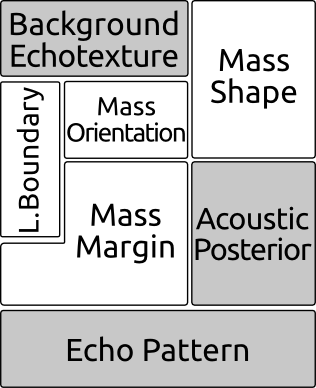
\includegraphics[width=1cm]{vcues}};}}\\
  %    &\multicolumn{2}{l}{\acs{rbf}-\acs{svm}}\\
  %    $V(\cdot,\cdot)$:&\multicolumn{2}{l}{Homogenity}\\
  %  \end{tabular}
  %};
  %\node[yshift=2pt,remember picture, overlay, nodeBase, mlStyle, fit= (mlInit) (mlFin)]{};
\node[draw, %below= 2pt of methodTech,
minimum width = 3.9cm,
  label={[label distance=-0.5cm,text depth=15pt,anchor=south, rotate=90]left:testing}
  ](testingNode){
    \begin{tabular}{lclclc}
      \multicolumn{2}{l}{Database size:} & \multicolumn{4}{l}{$16$} \\
      \multicolumn{2}{l}{\ac{gt}:}       & \multicolumn{4}{l}{multi-label} \\
      \multicolumn{2}{l}{Task:}          & \multicolumn{4}{l}{$\mathcal{L} = \{\text{lesion}, \overline{\text{lesion}}\}$} \\
      \multicolumn{2}{l}{Trainning:}     & \multicolumn{4}{l}{Leave-one-Patient-Out}\\
      \ac{aov}:      & .623                                                                               & \acs{fpr}: & .4 & \acs{fnr}: & .008
    \end{tabular}
    };
%  \node[
%        draw=red,
%        minimum width=\textwidth,
%        fit=(current bounding box.north west) (current bounding box.south east),
%      ]at (current bounding box.center){};
\end{tikzpicture}

};
\end{tikzpicture}
 }
    %\caption{{\small comparison}}
    \label{fig:surveyResults:comparison}
  \end{subfloat}
  \caption{Quantitative results compilation and comparison}
  \label{fig:surveyResults}
\end{figure*}

The proposed methodology is evaluated using a dataset of 16 \ac{bus} images presenting a single lesion of variable extension.
The size of the lesions ranges from under $1/100$ to over $1/5$ of the image size.
The dataset is composed of cysts, \acp{fa}, \acp{dic} and \acp{ilc}.
Every image has accompanying multi-label \ac{gt} delineating all the depicted structures.
This dataset is now publicly available at \texttt{http://visor.udg.edu/dataset/\#breast}

The lack of publicly available data and source code, limits the comparison between the
different methods.
For this study, the results published by the other authors have been collected and expressed in terms of \ac{aov} in order to share a common metric.
Further details can be found in~\cite{massich2013phd} and summarized in Fig.\,\ref{fig:surveyResults}.

Figure~\ref{fig:surveyResults} is divided into three main parts: (i) a table on the top summarizes the core stages of each study framework, (ii) a legend box on the right side informs our testing setup and, (iii) a comparison of the different metrics in a radial manner. An extra element is also represented in this radial representation: a blue swatch delimited by two blue dashed lines. The boundaries of this swatch correspond to the performance of some expert radiologists based on an inter- and intra-observer experiments carried out by Pons et al.~\cite{gerard2013}.
It is interesting to note that some methodologies outperform this swatch.
A publicly available dataset should allow a better comparison in that regard.

The results point out the inherent capabilities of \ac{ml} to cope with data scalability and variability, induce its usage in conjunction with larger datasets.
Whereas, \ac{acm} methodologies show its effectiveness to model the boundary in a natural manner.
% The ability of \ac{ml} to cope with data variability, as well as its need of data, explains why these methodologies
% have been tested, whereas the ability of \ac{acm} methods in constraining the boundary lead to slightly better results in terms of \ac{aov}.

For our proposed framework, the performance in terms of \ac{aov} lies within the state-of-the-art despite its final delineation
limited by the capacity of the super-pixels to snap the desired boundary.
Figure~\ref{fig:results} shows some qualitative results where there are limitations of labeling super-pixels when compared with hand-drawn \ac{gt}.
Figure~\ref{fig:results} also illustrates the influence of the pair-wise term.
%depicts the differences between the delineation resulting from a proper labeling of the super-pixels and the one from the \ac{gt}.

%The iconography used for the table, relates methodology stages, the technology used and if the stages have been treated separately or as a single processing.
%The figure, also arranges the information in a radial manner for direct visual comparison.



%Comparing these results, the inconvenience of unexciting public data can be obviously highlighted, since that several of these results outperform the manual delineations performed in Pons et al.~\cite{gerard2013} on the dataset here used.


% Figure~\ref{fig:results} shows qualitative results, whereas the quantitative results from the best configuration are reported as a table in Fig.\,\ref{fig:surveyResults}. %~\cite{massich2013phd}.

%Despite the fact that a \ac{fpr} of $0.4$ seems significant, based on our experiments most of the images produce no \ac{fp} lesions.
%However, images with \ac{fp} lesions, are likely to produce more several of them as shown in \cref{fig:results}c-e.
%The amount of \ac{fp} lesions can be trimmed by applying a higher cost in the pairwise therm (compare \cref{fig:resuts:smallPWterm} and \cref{fig:results:bigPWterm}.
%Nevertheless, a severe increasing of the pairwise cost also increases the \ac{fnr} since some lesions are missed due to over-smoothing. %~\cite{massich2013phd}.
%The situation of having a larger \ac{fnr} is less desirable than reducing the \ac{fpr}.
%The \ac{fnr} reported in \cref{fig:surveyResults:method} is caused by an image within the dataset that its lesion is fully contained in a single super-pixel and still around $20\%$ of this super-pixel's area is healty tissue.

% Due to the lack of publicly available data and source code, there is no manner to perform a comparison further apart of compiling the results reported in the literature.
% Based on \emph{******** et al.} the state-of-the-art methodologies found in the literature, the results are summarized in Fig.\,\ref{fig:surveyResults} and are reported in terms of \ac{aov} for comparison purposes. The references equivalence can be found in~\cite{massich2013phd}
%compiles relevant metholodologies relevant methodologies found in the literature
%The table in \Cref{fig:surveyResults:survey} complies the evaluation reported by the authors of the most relevant methodologies found in the literature. %~\cite{massich2013phd}.
%Details about the methodologies proposed in the literature can also be found in the aforesaid table.
%Specifically it is detailed the category of technique been used for detecting the lesions, segmenting it and post-process the delineations (if any).
%The studied categories are: \ac{ml}, \ac{acm} and others.
%if the those stages are treated as independent and connected in a daisy-chain fashion, or otherwise the stages are addressed in an atomic manner.


%\Cref{fig:surveyResults:comparison} renders the information present in \cref{fig:surveyResults:survey} and \cref{fig:surveyResults:method} in a visual manner compare all the results at once.
%The methodologies arranged in a radial fashion and grouped by its most representative technology category.
%In red it can be found a small, medium and large categorization of the dataset reported for testing.
%The concentric circles represent \ac{aov}.
%The blue line correspond to the \ac{aov} results reported in the literature, whereas the black line indicates the \ac{aov} our framework scored in our testing.

%\footnote{The dataset used for testing the framework here proposed corresponds to the subset of images used by Pons et al.~\cite{gerard2013} that have accompanying multi-labelled \ac{gt}.}.

%%% Local Variables:
%%% mode: latex
%%% TeX-master: "../../master.tex"


% \section{Conclusions}\label{sec:con}
% The work presented here addresses the automatic classification of \ac{sdoct} data to identify subjects with \ac{dme} versus normal.
% Based on the reported results, the low level volume 3D features and high level 2D features using patches achieve the most desirable results in the experimental setup presented here.
% The comparison against different datasets and methodologies, highlights that:
% regardless of using low or high level representations, volume signatures derived from \ac{lbp} texture show high discriminative power for distinguishing \ac{dme} vs normal volumes.

{\small
\printbibliography
}

\end{document} 
